\begin{dang}{Xác định góc và tính tích vô hướng của hai véctơ}
\end{dang}
\boxmini{BÀI TẬP TỰ LUẬN}
\setcounter{vd}{0}
\begin{vd}
	Cho hình lập phương $ ABCD.A'B'C'D' $ có cạnh bằng 5. 
	\begin{tasks}
		\task Tìm góc giữa các cặp véc-tơ sau: $\vec{AC}$ và $\vec{AB}$; $\vec{AC}$ và $\vec{B'D'}$;  $\vec{AC}$ và $\vec{CD}$; $\vec{AD'}$ và $\vec{BD}$.
		\task Tính các tích vô hướng $\vec{AC}\cdot \vec{AB}$;  $\vec{AC}\cdot \vec{B'D'}$; $\vec{AD'}\cdot\vec{BD}$;
		\task Chứng minh $\vec{AC'}$ vuông góc với $\vec{BD}$.
	\end{tasks}
	\loigiai{
	\immini{\begin{enumerate}[a)]
			\item Ta có : 
			\begin{itemize}
				\item [$\bullet$] $\left( \vec{AC},\vec{AB}\right)=\widehat{CAB}=45^\circ$
				\item [$\bullet$] $\left(\vec{AC},\vec{B'D'}\right)=\left(\vec{AC},\vec{BD}\right)=90^\circ$. 
				\item [$\bullet$] $\left(\vec{AC},\vec{CD}\right)=\left(\vec{CE},\vec{CD}\right)=180^\circ-45^\circ=135^\circ$ (E là điểm đối xứng của $A$ qua $C$). 
				\item [$\bullet$] $ \vec{AD'}=\vec{BC'} \Rightarrow \left(\vec{AD'},\vec{BD}\right)=\left(\vec{BC'},\vec{BD}\right)=\widehat{C'BD}$.
				Lại có, tam giác $ C'BD $ là tam giác đều nên $ \widehat{C'BD}=60^\circ\Rightarrow \left(\vec{AD'},\vec{BD}\right)=60^\circ $.
			\end{itemize}
			\item Ta có $AC=BD=B'D'=5\sqrt{2}$. Suy ra
			\begin{itemize}
				\item [$\bullet$] $\vec{AC}\cdot \vec{AB}=AC.AB.\cos45^\circ =25$.
				\item [$\bullet$] Do $AC$ vuông góc $B'D'$ nên $\vec{AC}\cdot \vec{B'D'}=0$.
				\item [$\bullet$] $\vec{AD'}\cdot \vec{BD}=AD'.BD.\cos60^\circ =5\sqrt{2}.5\sqrt{2}.\dfrac{1}{2}=25$.
			\end{itemize}
			\item Ta cần chứng minh $\vec{AC'}\cdot \vec{BD}=0$.\\
			Ta có: $\vec{AC'}=\vec{AB}+\vec{AD}+\vec{AA'}$ và $\vec{BD}=\vec{AD}-\vec{AB}$ nên
				\begin{eqnarray*}
				\vec{AC'}\cdot \vec{BD}
				&=&\left( \vec{AB}+\vec{AD}+\vec{AA'}\right)\cdot \left(\vec{AD}-\vec{AB} \right) \\
				&=&\vec{AB}.\vec{AD}-\vec{AB}^2+\vec{AD}^2-\vec{AD}.\vec{AB}+\vec{AA'}.\vec{AD}-\vec{AA'}.\vec{AB}=5^2-5^2=0
			\end{eqnarray*}
		Suy ra $\vec{AC'}$ vuông góc với $\vec{BD}$.
		\end{enumerate}}{
	\begin{tikzpicture}[scale=0.6, font=\footnotesize, line join=round, line cap=round]
		\def\h{4}
		\foreach \x\y\t in {0/0/A,-1/-1.1/B,2.6/-1.1/C}
		\coordinate (\t) at (\x,\y);
		\coordinate (D) at ($(A)+(C)-(B)$);
		\coordinate (A') at ($(A)+(0,3.2)$);
		\coordinate (B') at ($(B)+(0,3.2)$);
		\coordinate (C') at ($(C)+(0,3.2)$);
		\coordinate (D') at ($(D)+(0,3.2)$);
		\coordinate (E) at ($2*(C)-(A)$);
		\draw (B')--(A')--(D')--(C')--(B')--(B)--(C)--(D)--(D') (C')--(C)--(E);
		\draw[dashed](B)--(A)--(D) (A)--(A') (A)--(C);
		\foreach \t/\g in {A/170,B/-150,C/-100,D/0,A'/100,B'/170,C'/-20,D'/50,E/0}
		\draw[fill=black] (\t) circle(1pt)
		node[shift={(\g:7pt)}]{$\t$};
	\end{tikzpicture}
	}
	}
\end{vd}
\dongcham{31}
\begin{vd}%[2H2H1-3]
	Cho tứ diện đều $ABCD$ có cạnh bằng $a$ và $M$ là trung điểm của $CD$.
	\begin{listEX}[1]
		\item Tính các tích vô hướng $\vec{AB} \cdot \vec{AC}$, $\vec{AB} \cdot \vec{AM}$.
		\item Tính góc $(\vec{AB}, \vec{CD})$.
	\end{listEX}
	\loigiai{
		\begin{enumerate}
			\item Ta có $\begin{aligned}[t]
				\vec{AC} \cdot \vec{AC}	&= |\vec{AB}| \cdot |\vec{AC}| \cdot \cos (\vec{AB},\vec{AC})\\
				&= AB \cdot AC \cdot \cos \widehat{BAC}\\
				&= a \cdot a \cdot \cos {60^0}\\
				&= \frac{a^2}{2}.
			\end{aligned}$\\
			Tương tự ta cũng có $\vec{AB} \cdot \vec{AD} = \dfrac{a^2}{2}$.
			\immini{
				Ta lại có $\vec{AM} = \dfrac{1}{2}(\vec{AC} + \vec{AD})$, suy ra
				\[ \vec{AB} \cdot \vec{AM} = \vec{AB} \cdot \frac{1}{2}(\vec{AC} +\vec{AD}) = \frac{1}{2}(\vec{AB} \cdot \vec{AC} + \vec{AB} \cdot \vec{AD}) = \frac{1}{2}\left(\frac{a^2}{2} + \frac{a^2}{2}\right) = \frac{a^2}{2}.\]
				\item Ta có $\vec{AB} \cdot \vec{CD}=(\vec{AM}+\vec{MB}) \cdot \vec{CD}=\vec{AM} \cdot \vec{CD} +\vec{MB} \cdot \vec{CD}$.\\
				Mà $AM$, $BM$ là trung tuyến của các tam giác đều $ACD$, $BCD$ nên $\vec{AM} \perp \vec{CD}, \vec{MB} \perp \vec{CD}$.\\
				Suy ra $\vec{AM} \cdot \vec{CD} = \vec{MB} \cdot \vec{CD} = 0$.\\
				Từ các kết quả trên ta có $\vec{AM} \cdot \vec{CD}=0$.
				Suy ra $(\vec{AB}, \vec{CD})=90^\circ$.
			}{
				\begin{tikzpicture}[scale=1, font=\footnotesize, line join=round, line cap=round, >=Stealth]
					\def\a{3}
					\path 
					(0:0) coordinate (B)
					(5:\a) coordinate (D)
					($(D)+(-135:\a/2)$) coordinate (C)
					($(B)+(65:\a)$) coordinate (A)
					($(C)!.5!(D)$) coordinate (M)
					;
					\draw[->] (A)--(D);
					\draw[->] (A)--(C);
					\draw[->] (A)--(B);
					\draw[->] (A)--(M);
					\draw[dashed] (B)--(D);
					\draw (B)--(C)--(D);
					\foreach \x/\g in {A/90,B/180,C/-90,D/0,M/0}
					\draw[fill=black] 	(\x) circle (.5pt)
					($(\g:.3)+(\x)$) node {$\x$};	
				\end{tikzpicture}
			}
		\end{enumerate}
	}
\end{vd}
\dongcham{18}
\begin{vd}
	\immini{Cho biết công $A$ (đơn vị: $J$) sinh bởi lực $\vec{F}$ tác dụng lên một vật được tính bằng công thức $A = \vec{F}\cdot\vec{d}$, trong đó $\vec{d}$ là vectơ biểu thị độ dịch chuyển của vật (đơn vị của $\left|\vec{d}\right|$ là m) khi chịu tác dụng của lực $\vec{F}$.
	}{
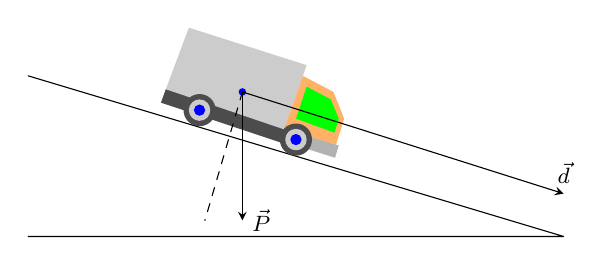
\begin{tikzpicture}[scale=0.68,font=\footnotesize, line join=round, line cap=round, >=stealth]
	\def\xe{orange!60}
	\def\den{red}
	\draw (0,3)--(10,0) (0,0)--(10,0);
	\fill[black!30] (2.48,2.5)--(2.57,2.75)--(5.8,1.7)--(5.73,1.47)--cycle ;
	\fill[black!70] (2.48,2.5)--(2.57,2.75)--(5.2,2)--(5.18,1.6)--cycle ;
	\fill[black!20] (2.57,2.75)--(3,3.9)--(5.2,3.2)--(4.78,2)--cycle ;
	\fill[\xe] (4.78,2)--(5.13,3)--(5.7,2.7)--(5.9,2.2)--(5.75,1.72)--cycle ;
	\fill[green] (5.2,2.8)--(5.65,2.56)--(5.8,2.2)--(5.72,1.94)--(5,2.2)--cycle ;
	\fill[black!70] (3.2,2.36) circle (0.3) (5,1.81) circle (0.3) ;
	\fill[black!20] (3.2,2.36) circle (0.2) (5,1.81) circle (0.2) ;
	\fill[blue](3.2,2.36) circle (3pt) (5,1.81) circle (3pt) (4,2.7) circle (2pt) ;
	\draw[dashed] (4,2.7)--(3.3,0.3) ;
	\draw[->] (4,2.7)--(4,0.3) node[right] {$\vec{P}$};
	\draw[->] (4,2.7)--(10,0.8) node[above] {$\vec{d}$};
\end{tikzpicture} }
Một chiếc xe có khối lượng $1{,}5$ tấn đang đi xuống trên một đoạn đường dốc có góc nghiêng $5^\circ$ so với phương ngang. Tính công sinh bởi trọng lực $\vec{P}$ khi xe đi hết đoạn đường dốc dài $30$ m (làm tròn kết quả đến hàng đơn vị), biết rằng trọng lực $\vec{P}$ được xác định bởi công thức $\vec{P} = m\vec{g}$, với $m$ (đơn vị: kg) là khối lượng của vật và $\vec{g}$ là gia tốc rơi tự do có độ lớn $g = 9{,}8$ m/s$^2$.
	\loigiai{
		\begin{center}
			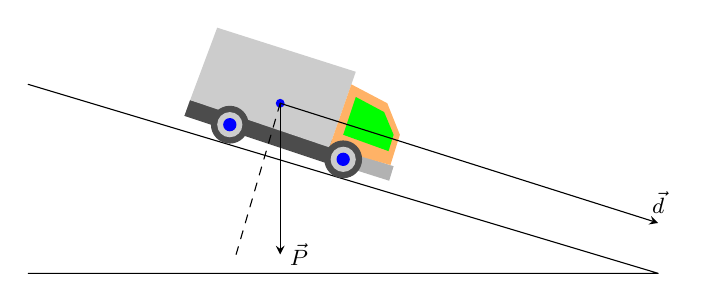
\begin{tikzpicture}[scale=0.8,font=\footnotesize, line join=round, line cap=round, >=stealth]
				\def\xe{orange!60}
				\def\den{red}
				\draw (0,3)--(10,0) (0,0)--(10,0);
				\fill[black!30] (2.48,2.5)--(2.57,2.75)--(5.8,1.7)--(5.73,1.47)--cycle ;
				\fill[black!70] (2.48,2.5)--(2.57,2.75)--(5.2,2)--(5.18,1.6)--cycle ;
				\fill[black!20] (2.57,2.75)--(3,3.9)--(5.2,3.2)--(4.78,2)--cycle ;
				\fill[\xe] (4.78,2)--(5.13,3)--(5.7,2.7)--(5.9,2.2)--(5.75,1.72)--cycle ;
				\fill[green] (5.2,2.8)--(5.65,2.56)--(5.8,2.2)--(5.72,1.94)--(5,2.2)--cycle ;
				\fill[black!70] (3.2,2.36) circle (0.3) (5,1.81) circle (0.3) ;
				\fill[black!20] (3.2,2.36) circle (0.2) (5,1.81) circle (0.2) ;
				\fill[blue](3.2,2.36) circle (3pt) (5,1.81) circle (3pt) (4,2.7) circle (2pt) ;
				\draw[dashed] (4,2.7)--(3.3,0.3) ;
				\draw[->] (4,2.7)--(4,0.3) node[right] {$\vec{P}$};
				\draw[->] (4,2.7)--(10,0.8) node[above] {$\vec{d}$};
			\end{tikzpicture} 
			%\includegraphics{hinhanh/H1.png} 
		\end{center}
		\noindent 
		Ta có $1{,}5$ tấn = $1~500$ kg.\\
		Độ lớn của trọng lực tác dụng lên chiếc xe là $\left|\vec{P}\right| = m \left|\vec{g}\right| = 1~500\cdot 9{,}8 = 14~700$ (N).\\
		Vectơ d biểu thị độ dịch chuyển của xe có độ dài là $\left|\vec{d}\right| = 30$ (m) và $ \left(\vec{P},\vec{d}\right)= 90^\circ - 5^\circ = 85^\circ$.\\
		Công sinh ra bởi trọng lực $\vec{P}$ khi xe đi hết đoạn đường dốc dài $30$ m là
		$$A=\vec{P}\cdot\vec{d}=\left|\vec{P}\right|\cdot\left|\vec{d}\right|\cdot\cos\left(\vec{P},\vec{d}\right) = 14~700\cdot 30\cdot \cos 85^\circ \approx 38~436~(J).$$
	}
\end{vd}
\dongcham{7}
\begin{vd}
	\immini{
		Một chất điểm $A$ nằm trên mặt phẳng nằm ngang $\left(\alpha\right)$, chịu tác động bởi ba lực $\vec{F}_1$, $\vec{F}_2$, $\vec{F}_3$. Các lực $\vec{F}_1$, $\vec{F}_2$ có giá nằm trong $\left(\alpha\right)$ và $\left(\vec{F}_1, \vec{F}_2\right)=135^\circ$, còn lực $\vec{F}_3$ có giá vuông góc với $\left(\alpha\right)$ và hướng lên trên. Xác định cường độ hợp lực của các lực $\vec{F}_1$, $\vec{F}_2$, $\vec{F}_3$ biết rằng độ lớn của ba lực đó lần lượt là $20$ N, $15$ N và $10$ N.
	}{
		\begin{tikzpicture}[line join=round, line cap = round, >=stealth, scale=0.75,font=\footnotesize]
			\path 
			(0,0) coordinate (A) 
			(-2,-1.5) coordinate (B) 
			(3,0) coordinate (C) 
			(0,3) coordinate (D) 
			; 
			\draw[->] (A)--(B) node[below] {$\vec{F}_1$}; 
			\draw[->] (A)--(C) node[below] {$\vec{F}_2$}; 
			\draw[->] (A)--(D) node[right] {$\vec{F}_3$};
			\draw pic[draw,angle eccentricity=1.2,angle radius=0.2cm]{right angle= D--A--C};
			\draw pic[draw,angle eccentricity=1.2,angle radius=0.2cm]{right angle= D--A--B};
			\draw pic[draw,angle eccentricity=1.2,angle radius=0.3cm]{angle= B--A--C};
			\draw ($(A)-(-0.3,0.6)$) node {$135^\circ$}; 
			\foreach \x/\g in {A/140} \fill[black](\x) circle (1pt) ($(\x)+(\g:4mm)$)node{$\x$}; 
		\end{tikzpicture} 
	}
	\loigiai{
		Gọi $\vec{F}$ là hợp lực của các lực $\vec{F}_1$, $\vec{F}_2$, $\vec{F}_3$, tức là $\vec{F}= \vec{F}_1+ \vec{F}_2+ \vec{F}_3$, ta có
		\allowdisplaybreaks 
		\begin{eqnarray*}
			\left|\vec{F}\right|^2 &=& \left(\vec{F}_1+ \vec{F}_2+ \vec{F}_3\right)^2\\
			&=& \vec{F}_1^2+ \vec{F}_2^2+ \vec{F}_3^2+ 2\vec{F}_1\cdot\vec{F}_2+ 2\vec{F}_2\cdot\vec{F}_3+ 2\vec{F}_3\cdot\vec{F}_1\\
			&=& 20^2+ 15^2+ 10^2+ 2\cdot 20\cdot 15\cdot\cos 135^\circ\\
			&=& 725-300\sqrt2.
		\end{eqnarray*}
		Vậy $\left|\vec{F}\right|= \sqrt{725-300\sqrt2} \approx 17{,}34$ (N).
	}
\end{vd}
\dongcham{11}
\boxmini{BÀI TẬP TRẮC NGHIỆM}
\ind{PHẦN I.} \inden{Câu trắc nghiệm nhiều phương án lựa chọn. Mỗi câu hỏi học sinh chỉ chọn một phương án.}\\
\setcounter{ex}{0}
\Opensolutionfile{ans}[ans/2H2-B1-d2-1]

\begin{ex} %[Word to LaTeX 3.2]
	Cho $\vec{a}$ và $\vec{b}$ là hai vectơ cùng hướng và đều khác vectơ $\vec{0}$. Mệnh đề nào sau đây đúng?
	\choice
	{$\vec{a}\cdot\vec{b}=0$}
	{$\vec{a}\cdot\vec{b}=-1$}
	{\True $\vec{a}\cdot\vec{b}=\left|{\vec{a}}\right|.\left|{\vec{b}}\right|$}
	{$\vec{a}\cdot\vec{b}=-\left|{\vec{a}}\right|.\left|{\vec{b}}\right|$}
	\loigiai{
		Do $\vec{a}$ và $\vec{b}$ là hai vectơ cùng hướng nên $\left(\vec{a},\vec{b}\right)=0^0\Rightarrow cos\left(\vec{a},\vec{b}\right)=1$. Vậy $\vec{a}.\vec{b}=\left|{\vec{a}}\right|.\left|{\vec{b}}\right|$}
\end{ex}
\cham{2}
\begin{ex} %[Word to LaTeX 3.2]
	Cho hai vectơ $\vec{a}$ và $\vec{b}$ khác $\vec{0}$. Xác định góc $\alpha $ giữa hai vectơ $\vec{a}$ và $\vec{b}$ khi $\vec{a}.\vec{b}=-\left|{\vec{a}}\right|.\left|{\vec{b}}\right| $.
	\choice
	{$\alpha =0^\circ$}
	{$\alpha =45^\circ$}
	{$\alpha =90^\circ$}
	{\True $\alpha =180^\circ$}
	\loigiai{
		Mà theo giả thiết $\vec{a}.\vec{b}=-\left|{\vec{a}}\right|.\left|{\vec{b}}\right|$, suy ra $\cos \left(\vec{a},\vec{b}\right)=-1\Rightarrow \left(\vec{a},\vec{b}\right)=180^0$}
\end{ex}
\cham{2}
\begin{ex}
	Cho hai vectơ $\overrightarrow{u}$ và $\overrightarrow{b}$ thỏa mãn $|\overrightarrow{u}|=8,|\overrightarrow{b}|=2$ và $\overrightarrow{u}.\overrightarrow{b}=8$. Góc giữa hai vectơ đã cho là
	\choice
	{ $30^\circ$ }
	{ \True $60^\circ$ }
	{ $135^\circ$ }
	{ $120^\circ$ }
	\loigiai{ 
		$\cos (\overrightarrow{u},\overrightarrow{b})=\dfrac{\overrightarrow{u}.\overrightarrow{b}}{|\overrightarrow{u}|.|\overrightarrow{b}|}=\dfrac{8}{8.2}=\frac{1}{2}$.
		
		Suy ra $(\overrightarrow{u},\overrightarrow{b})=60^\circ$. 
}\end{ex}
\cham{2}
\begin{ex}
	Cho hai vectơ $\overrightarrow{a}$ và $\overrightarrow{b}$ thỏa mãn $|\overrightarrow{a}|=7,|\overrightarrow{b}|=2$ và $\overrightarrow{a}.\overrightarrow{b}=7 \sqrt{2}$. Góc giữa hai vectơ đã cho là
	\choice
	{ $120^\circ$ }
	{ \True $45^\circ$ }
	{ $180^\circ$ }
	{ $30^\circ$ }
	\loigiai{ 
		$\cos (\overrightarrow{a},\overrightarrow{b})=\dfrac{\overrightarrow{a}.\overrightarrow{b}}{|\overrightarrow{a}|.|\overrightarrow{b}|}=\dfrac{7 \sqrt{2}}{7.2}=\frac{\sqrt{2}}{2}$.
		
		Suy ra $(\overrightarrow{a},\overrightarrow{b})=45^\circ$. 
}\end{ex}
\cham{2}
\begin{ex}
	\immini[thm]{Cho hình lập phương ${ABCD.A_1B_1C_1D_1}$. Góc giữa hai vectơ $\overrightarrow{B_1C_1}$ và $\overrightarrow{BD}$ bằng 
	\choice
	{ $135^\circ$ }
	{ \True $45^\circ$ }
	{ $120^\circ$ }
	{ $60^\circ$ }
}{
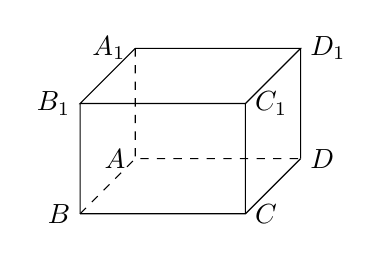
\begin{tikzpicture}[scale=0.7] 
	\coordinate (A) at (0,0)   node at (A) [left] {$A$};
	\coordinate (B) at (-1,-1) node at (B) [left] {$B$};
	\coordinate (C) at (2,-1)  node at (C) [right] {$C$};
	\coordinate (D) at (3,0)   node at (D) [right] {$D$};
	\coordinate (A_1) at (0,2)   node at (A_1) [left] {$A_1$};
	\coordinate (B_1) at (-1,1) node at (B_1) [left] {$B_1$};
	\coordinate (C_1) at (2,1)  node at (C_1) [right] {$C_1$};
	\coordinate (D_1) at (3,2)   node at (D_1) [right] {$D_1$};
	\draw [dashed] (B)--(A)--(D) (A_1)--(A);
	\draw (A_1)--(B_1)--(C_1)--(D_1)--(A_1) (B_1)--(B) (C_1)--(C) (D_1)--(D);
	\draw (B)--(C)--(D);
\end{tikzpicture}}
	\loigiai{ 
		Góc $(\overrightarrow{B_1C_1}, \overrightarrow{BD})=$ $45^\circ$. 
}\end{ex}
\cham{2}
\begin{ex}
	\immini[thm]{Cho hình lập phương $ABCD.A'B'C'D'$. Khẳng định nào sau đây là khẳng định \textbf{sai}?
		\choice
		{ $\left(\vec{A'C'},\vec{AD}\right)=45^\circ$}
		{$\left(\vec{A'C'},\vec{B'B}\right)=90^\circ$}
		{\True $\left(\vec{A'A}, \vec{CB'}\right)=45^\circ$}
		{$\left(\vec{AB},\vec{CD}\right)=180^\circ$}
	}{
		\begin{tikzpicture}[scale=0.5, font=\footnotesize,>=stealth]
			%Gán số liệu.
			\def\canhAD{3};\def\canhBA{2};\def\gocBAD{-130};\def\h{3};\def\xdinhA'{0};
			%Gán tọa độ.
			\coordinate (A) at (0,0);
			\coordinate (B) at ($(A)+(\gocBAD:\canhBA)$);
			\coordinate (C) at ($(B)+(0:\canhAD)$);
			\coordinate (D) at ($(A)+(0:\canhAD)$);
			\coordinate (A') at ($(A)+(\xdinhA',\h)$);
			\coordinate (B') at ($(B)+(\xdinhA',\h)$);
			\coordinate (C') at ($(C)+(\xdinhA',\h)$);
			\coordinate (D') at ($(D)+(\xdinhA',\h)$);
			%Vẽ khối lẳng trụ ABCD.A'B'C'D'.
			\draw (A')--(B')--(B)--(C)--(C')--(D')--cycle (B')--(C') (D')--(D)--(C) (A')--(C');
			\draw[dashed] (A)--(D) (A')--(A)--(B) (A)--(C);
			%Gán nhãn.
			\foreach \x/\y in {A/180, B/180, C/0, D/0, A'/180, B'/180, C'/0, D'/0}{\fill (\x) circle(1pt) ($(\x)+(\y:0.3cm)$) node{$\x$};}
	\end{tikzpicture}}
	\loigiai{
		\begin{itemize}
			\item [$\bullet$] Ta có $\left(\vec{A'C'},\vec{AD}\right)=\left(\vec{A'C'},\vec{A'D'}\right)=\widehat{C'A'D'}=45^\circ$.
			\item [$\bullet$] $\left(\vec{A'C'},\vec{B'B}\right)=\left(\vec{A'C'},\vec{A'A}\right)=\widehat{AA'C'}=90^\circ$.
			\item [$\bullet$] Ta có $\vec{B'B}=\vec{A'A}$, suy ra\\
			$\left(\vec{A'A},\vec{CB'}\right)=\left(\vec{B'B},\vec{CB'}\right)=180^{\circ}-\widehat{BB'C}=180^{\circ}-45^{\circ}=135^{\circ}$
			\item [$\bullet$] $\vec{AB}$ ngược hướng với $\vec{CD}$ nên $\left(\vec{AB},\vec{CD}\right)=180^\circ$.
		\end{itemize}
	}
\end{ex} \cham{2}

\begin{ex}
Cho tứ diện đều $ABCD$, Gọi $M$, $N$ lần lượt là trung điểm các cạnh $AB$, $AC$. Hãy tính góc giữa hai vectơ $\vec{MN}$ và $\vec{BD}$.
		\choice
		{$ \left(\vec{MN}, \vec{BD} \right) = 150^\circ$}
		{$ \left(\vec{MN}, \vec{BD} \right) = 120^\circ$}
		{$ \left(\vec{MN}, \vec{BD} \right) = 30^\circ$}
		{\True $ \left(\vec{MN}, \vec{BD} \right) = 60^\circ$}
	\loigiai{
		\immini{Xét tam giác $ABC$ có $M$, $N$ là trung điểm của $AB$, $AC$ nên $MN$ là đường trung bình của tam giác $ABC$. Do đó $MN \parallel BC$.\\
			Ta có $ \left(\vec{MN}, \vec{BD} \right)= \left(\vec{BC}, \vec{BD} \right) = \widehat{CBD}$. \\
			Vì $ABCD$ là tứ diện đều nên $BC=CD=DB$. Do đó tam giác $BCD$ đều suy ra $\widehat{CBD} = 60^\circ$.\\
			Vậy $ \left(\vec{MN}, \vec{BD} \right) = 60^\circ$.}
		{\begin{tikzpicture}[scale=0.55, font=\footnotesize, line join=round, line cap=round]
				\foreach \x\y\t in {0/0/B,6/0/D,1.5/-2/C,1.5/5/A}
				\coordinate (\t) at (\x,\y);
				\coordinate (M) at ($(A)!1/2!(B)$);
				\coordinate (N) at ($(A)!1/2!(C)$);
				\draw (A)--(B)--(C)--(D)--(A)--(C);
				\draw[dashed,-stealth,blue,very thick] (B)--(D);
				\draw[-stealth,blue,very thick](M)--(N);
				\foreach \t/\g in {A/90,B/180,C/-90,D/0,M/180,N/0} \draw (\t) node[shift={(\g:10pt)}]{$\t$};
		\end{tikzpicture}}
	}
\end{ex} \cham{5} 

\begin{ex}
	\immini[thm]{Cho hình chóp $S. A B C D$ có đáy $A B C D$ là hình bình hành và mặt bên $S A B$ là tam giác đều. Tính góc giữa hai vectơ $\vec{D C}$ và $\vec{B S}$.
		\haicot
		{\True $\left(\vec{D C}, \vec{B S}\right)=120^{\circ}$}
		{$\left(\vec{D C}, \vec{B S}\right)=60^{\circ}$}
		{$\left(\vec{D C}, \vec{B S}\right)=90^{\circ}$}
		{$\left(\vec{D C}, \vec{B S}\right)=150^{\circ}$}
	}{
		\begin{tikzpicture}[scale=0.8, font=\footnotesize,>=stealth]
			%Gán số liệu.
			\def\canhAD{4};\def\canhBA{2};\def\gocBAD{-130};\def\h{2};\def\xdinhS{-1};
			%Gán tọa độ.
			\coordinate (A) at (0,0);
			\coordinate (B) at ($(A)+(\gocBAD:\canhBA)$);
			\coordinate (C) at ($(B)+(0:\canhAD)$);
			\coordinate (D) at ($(A)+(0:\canhAD)$);
			\coordinate (S) at ($(A)+(\xdinhS,\h)$);
			\draw (B)--(S)--(C)--cycle (S)--(D)--(C);
			\draw[dashed] (A)--(D) (S)--(A)--(B);
			\foreach \x/\y in {A/180,B/-90,C/-90,D/0,S/90}{\fill (\x) circle(1pt) ($(\x)+(\y:0.3cm)$) node{$\x$};}
		\end{tikzpicture}
	}
	\loigiai{
		\immini{Vì $A B C D$ là hình bình hành nên $A B \parallel D C$.\\
			Trên tia $A B$ lấy điểm $E$ sao cho $\vec{B E}=\vec{D C}$ (Hình $2.20$). Ta có
			$$
			\left(\vec{D C}, \vec{B S}\right)=\left(\vec{B E}, \vec{B S}\right)=\widehat{E B S}=180^{\circ}-60^{\circ}=120^{\circ}.
			$$
			Vậy $\left(\vec{D C}, \vec{B S}\right)=120^{\circ}$.
		}{
			\begin{tikzpicture}[scale=0.8, font=\footnotesize,>=stealth]
				%Gán số liệu.
				\def\canhAD{4};\def\canhBA{2};\def\gocBAD{-130};\def\h{2};\def\xdinhS{-1};
				%Gán tọa độ.
				\coordinate (A) at (0,0);
				\coordinate (B) at ($(A)+(\gocBAD:\canhBA)$);
				\coordinate (C) at ($(B)+(0:\canhAD)$);
				\coordinate (D) at ($(A)+(0:\canhAD)$);
				\coordinate (S) at ($(A)+(\xdinhS,\h)$);
				\coordinate (E) at ($(B)!-1!(A)$);
				%Vẽ khối chóp S.ABCD.
				\draw (B)--(S)--(C)--cycle (S)--(D)--(C);
				\draw[dashed] (A)--(D) (S)--(A)--(B);
				\draw[->] (B)--(E);
				\draw[->] (D)--(C);
				%	%Gán nhãn.
				\draw pic["$60^\circ$",draw,angle eccentricity=1.6,angle radius=0.5cm]{angle=A--B--S};
				\draw pic["$120^\circ$",draw,double,angle eccentricity=1.7,angle radius=0.4cm]{angle=S--B--E};
				\foreach \x/\y in {A/180,B/-90,C/-90,D/0,S/90, E/90}{\fill (\x) circle(1pt) ($(\x)+(\y:0.3cm)$) node{$\x$};}
			\end{tikzpicture}
		}
	}
\end{ex} \cham{4}


\begin{ex}
	Cho hai vectơ $\overrightarrow{u}$ và $\overrightarrow{v}$ thỏa mãn $|\overrightarrow{u}|=8,|\overrightarrow{v}|=8$ và góc giữa hai vectơ bằng ${60}^\circ$.Tính tích vô hướng $\overrightarrow{u}.\overrightarrow{v}$.\ 
	\choice
	{ \True ${32}$ }
	{ ${32 \sqrt{3}}$ }
	{ ${64 \sqrt{3}}$ }
	{ ${64}$ }
	\loigiai{ 
		$\overrightarrow{u}.\overrightarrow{v}=8.8.\cos 60^\circ={32}$. 
}\end{ex}
\cham{2}
\begin{ex}
	\immini[thm]{Cho hình chóp $S.A B C D$ có đáy $A B C D$ là hình bình hành. Mặt bên $A S B$ là tam giác vuông cân tại $S$ và có cạnh $A B=a$. Tính $\vec{D C} \cdot \vec{A S}$.
		\haicot
		{$\dfrac{a^2}{4}$}
		{$-\dfrac{a^2}{4}$}
		{$-\dfrac{a^2}{2}$}
		{\True $\dfrac{a^2}{2}$}}{
		\begin{tikzpicture}[scale=0.7, font=\footnotesize,>=stealth]
			\def\canhAD{4};\def\canhBA{2};\def\gocBAD{-130};\def\h{2};\def\xdinhS{-1};
			%Gán tọa độ.
			\coordinate (A) at (0,0);
			\coordinate (B) at ($(A)+(\gocBAD:\canhBA)$);
			\coordinate (C) at ($(B)+(0:\canhAD)$);
			\coordinate (D) at ($(A)+(0:\canhAD)$);
			\coordinate (S) at ($(A)+(\xdinhS,\h)$);
			\draw (B)--(S)--(C)--cycle (S)--(D)--(C);
			\draw[dashed] (A)--(D) (S)--(A)--(B);
			\draw[->] (D)--(C);
			%\draw pic["$45^\circ$",draw,angle eccentricity=1.6,angle radius=0.3cm]{angle=S--A--B};
			\foreach \x/\y in {A/60,B/-90,C/-90,D/0,S/90}{\fill (\x) circle(1pt) ($(\x)+(\y:0.3cm)$) node{$\x$};}
	\end{tikzpicture}}
	\loigiai{
		\immini{$\vec{D C} \cdot \vec{A S}=\vec{A B} \cdot \vec{A S}=\left|\vec{A B}\right| \cdot\left|\vec{A S}\right| \cdot \cos \left(\vec{A B}, \vec{A S}\right)=a \cdot \dfrac{a \sqrt{2}}{2} \cdot \cos 45^{\circ}=\dfrac{a^2}{2}$.
		}{
			\begin{tikzpicture}[scale=0.9, font=\footnotesize,>=stealth]
				\def\canhAD{4};\def\canhBA{2};\def\gocBAD{-130};\def\h{2};\def\xdinhS{-1};
				%Gán tọa độ.
				\coordinate (A) at (0,0);
				\coordinate (B) at ($(A)+(\gocBAD:\canhBA)$);
				\coordinate (C) at ($(B)+(0:\canhAD)$);
				\coordinate (D) at ($(A)+(0:\canhAD)$);
				\coordinate (S) at ($(A)+(\xdinhS,\h)$);
				\draw (B)--(S)--(C)--cycle (S)--(D)--(C);
				\draw[dashed] (A)--(D) (S)--(A)--(B);
				\draw[->] (D)--(C);
				\draw pic["$45^\circ$",draw,angle eccentricity=1.6,angle radius=0.3cm]{angle=S--A--B};
				\foreach \x/\y in {A/60,B/-90,C/-90,D/0,S/90}{\fill (\x) circle(1pt) ($(\x)+(\y:0.3cm)$) node{$\x$};}
		\end{tikzpicture}}
	}
\end{ex} \cham{2}

\begin{ex}
	\immini[thm]{Cho hình lập phương $ABCD.EFGH$ có các cạnh bằng $ a $. Tính $\vec{AB}\cdot\vec{EG}$.
		\haicot
		{$a^2\sqrt{2}$}
		{\True $a^2$}
		{$\dfrac{a^2\sqrt{2}}{2}$}
		{$a^2\sqrt{3}$}}{
		\begin{tikzpicture}[scale=0.5, font=\footnotesize, line join=round, line cap=round, >=stealth]
			\coordinate (A) at (0,0);
			\coordinate (B) at (-1.5,-1.5);
			\coordinate (D) at (3,0);
			\coordinate (A') at (0,3);
			\coordinate (C) at ($(D)+(B)-(A)$);
			\coordinate (B') at ($ (A')-(A)+(B) $);
			\coordinate (C') at ($ (A')-(A)+(C) $);
			\coordinate (D') at ($ (A')-(A)+(D) $);
			\draw (B)--(C)--(C')--(B')--cycle (A')--(B')--(C')--(D')--cycle (C)--(D)--(D') (C)--(D);
			\draw[dashed] (B)--(A)--(D) (A)--(A');
			\draw[dashed] (A)--(C);
			\draw[](A')--(C');
			\foreach \p/\t/\q in {A/A/150,B/B/-90,C/C/-90,D/D/30, A'/E/90, B'/F/180, C'/G/-30, D'/H/90} \draw[black,fill=white] (\p) circle(0.8pt)node[shift={(\q:6pt)}]{\color{black}$\t$};
	\end{tikzpicture}}
	\loigiai{
		\immini
		{
			Ta có $\vec{AB}\cdot\vec{EG}=\vec{AB}\cdot\vec{AC}=AB\cdot AC\cdot\cos45^\circ=a\cdot a\sqrt{2}\cdot\dfrac{\sqrt2}{2}=a^2$.
		}
		{
			\begin{tikzpicture}[scale=0.5, font=\footnotesize, line join=round, line cap=round, >=stealth]
				\coordinate (A) at (0,0);
				\coordinate (B) at (-1.5,-1.5);
				\coordinate (D) at (3,0);
				\coordinate (A') at (0,3);
				\coordinate (C) at ($(D)+(B)-(A)$);
				\coordinate (B') at ($ (A')-(A)+(B) $);
				\coordinate (C') at ($ (A')-(A)+(C) $);
				\coordinate (D') at ($ (A')-(A)+(D) $);
				\draw (B)--(C)--(C')--(B')--cycle (A')--(B')--(C')--(D')--cycle (C)--(D)--(D') (C)--(D);
				\draw[dashed] (B)--(A)--(D) (A)--(A');
				\draw[->,dashed] (A)--(C);
				\draw[->](A')--(C');
				\foreach \p/\t/\q in {A/A/150,B/B/-90,C/C/-90,D/D/30, A'/E/90, B'/F/180, C'/G/-30, D'/H/90} \draw[black,fill=white] (\p) circle(0.8pt)node[shift={(\q:6pt)}]{\color{black}$\t$};
			\end{tikzpicture}
		}
	}
\end{ex} \cham{2}

\begin{ex}
	\immini[thm]{Cho hình lập phương $ABCD.A'B'C'D'$ có cạnh bằng $a$. Tính $ \vec{A B'} \cdot \vec{A' C'}$.
		\haicot
		{$\dfrac{a^2}{2}$}
		{$-a^2$}
		{\True $a^2$}
		{$-\dfrac{a^2}{2}$}
	}{\hspace{1.5cm}
		\begin{tikzpicture}[scale=0.55, font=\footnotesize,>=stealth]
			%Gán số liệu.
			\def\canhAD{3};\def\canhBA{2};\def\gocBAD{-130};\def\h{3};\def\xdinhA'{0};
			%Gán tọa độ.
			\coordinate (A) at (0,0);
			\coordinate (B) at ($(A)+(\gocBAD:\canhBA)$);
			\coordinate (C) at ($(B)+(0:\canhAD)$);
			\coordinate (D) at ($(A)+(0:\canhAD)$);
			\coordinate (A') at ($(A)+(\xdinhA',\h)$);
			\coordinate (B') at ($(B)+(\xdinhA',\h)$);
			\coordinate (C') at ($(C)+(\xdinhA',\h)$);
			\coordinate (D') at ($(D)+(\xdinhA',\h)$);
			%\coordinate (F) at ($(A)!-1!(E)$);
			%\draw pic[draw,angle radius=0.3cm]{right angle=B'--H--E};
			%Vẽ khối lẳng trụ ABCD.A'B'C'D'.
			\draw (A')--(B')--(B)--(C)--(C')--(D')--cycle (B')--(C') (D')--(D)--(C) (A')--(C') ;
			\draw[dashed] (A)--(D) (A')--(A)--(B) (A)--(C) (A)--(B') (B)--(D) ;
			%Gán nhãn.
			\foreach \x/\y in {A/180, B/-90, C/0, D/0, A'/180, B'/180, C'/0, D'/0}{\fill (\x) circle(1pt) ($(\x)+(\y:0.3cm)$) node{$\x$};}
	\end{tikzpicture}}
	\loigiai{
		Ta có $A'C'=AC$.\\
		Vì $AB'=AC=B'C=a\sqrt{2}$ nên tam giác $AB'C$ đều. Suy ra $\widehat{B'AC}=60^\circ$.\\
		Ta có $\begin{aligned}[t]
			\vec{A B'} \cdot \vec{A' C'}&\ =\left|\vec{AB'}\right|\cdot\left|\vec{A'C'}\right|\cdot\cos \left(\vec{AB'},\vec{A'C'}\right)\\
			&\ = AB'\cdot A'C' \cdot \cos \left(\vec{AB'}, \vec{AC}\right)\\
			&\ = AB'\cdot A'C' \cdot \cos \widehat{B'AC}\\
			&\ = a\sqrt{2}\cdot a\sqrt{2}\cdot \cos 60^\circ= a^2.
		\end{aligned}$
	}
\end{ex} \cham{3}

\begin{ex}
	\immini[thm]{Cho hình lập phương $ABCD.A'B'C'D'$ có cạnh bằng $a$. Tính $\vec{A B'} \cdot \vec{B D} $.
		\haicot
		{$\dfrac{a^2}{2}$}
		{\True$-a^2$}
		{ $a^2$}
		{$-\dfrac{a^2}{2}$}
	}{\hspace{1.5cm}
		\begin{tikzpicture}[scale=0.7, font=\footnotesize,>=stealth]
			%Gán số liệu.
			\def\canhAD{3};\def\canhBA{2};\def\gocBAD{-130};\def\h{3};\def\xdinhA'{0};
			%Gán tọa độ.
			\coordinate (A) at (0,0);
			\coordinate (B) at ($(A)+(\gocBAD:\canhBA)$);
			\coordinate (C) at ($(B)+(0:\canhAD)$);
			\coordinate (D) at ($(A)+(0:\canhAD)$);
			\coordinate (A') at ($(A)+(\xdinhA',\h)$);
			\coordinate (B') at ($(B)+(\xdinhA',\h)$);
			\coordinate (C') at ($(C)+(\xdinhA',\h)$);
			\coordinate (D') at ($(D)+(\xdinhA',\h)$);
			%\coordinate (F) at ($(A)!-1!(E)$);
			%\draw pic[draw,angle radius=0.3cm]{right angle=B'--H--E};
			%Vẽ khối lẳng trụ ABCD.A'B'C'D'.
			\draw (A')--(B')--(B)--(C)--(C')--(D')--cycle (B')--(C') (D')--(D)--(C) (A')--(C') ;
			\draw[dashed] (A)--(D) (A')--(A)--(B) (A)--(C) (A)--(B') (B)--(D) ;
			%Gán nhãn.
			\foreach \x/\y in {A/180, B/-90, C/0, D/0, A'/180, B'/180, C'/0, D'/0}{\fill (\x) circle(1pt) ($(\x)+(\y:0.3cm)$) node{$\x$};}
	\end{tikzpicture}}
	\loigiai{
		Ta có $ABCD.A'B'C'D$ là hình lập phương nên $\heva{&AA'\perp AB\\ &AB\perp BC\\ &\vec{AD}=\vec{BC}\\
			&\vec{AB'}=\vec{AA'}+\vec{AB}\\ &\vec{BD}=\vec{BA}+\vec{BC}.}$\\
		Khi đó $\begin{aligned}[t]
			\vec{A B'} \cdot \vec{B D}&\ =\left(\vec{AA'}+\vec{AB}\right)\cdot \left(\vec{BA}+\vec{BC}\right)\\
			&\ =\vec{AA'}\cdot \vec{BA} +\vec{AA'}\cdot\vec{BC}+\vec{AB}\cdot\vec{BA}+\vec{AB}\cdot \vec{BC}.\\
			&\ = 0 + 0 - AB^2 + 0 =-a^2.
		\end{aligned}$
	}
\end{ex} \cham{3}

\begin{ex}
	\immini[thm]{Cho hình chóp tứ giác đều $S . A B C D$ có độ dài tất cả các cạnh bằng $a$. Tính $\vec{A S} \cdot \vec{B C}$.
		\haicot
		{$-\dfrac{a^2}{4}$}
		{\True $\dfrac{a^2}{2}$}
		{$-\dfrac{a^2}{2}$}
		{$\dfrac{a^2}{4}$}
	}{
		\begin{tikzpicture}[line join=round, line cap = round, >=stealth, scale=.7,font=\footnotesize]
			\def\a{4}
			\def\h{3.5}
			\path 	(0:0) coordinate (A)
			++(0:\a) coordinate (D)
			++(-150:\a/2) coordinate (C)
			($(A)+(C)-(D)$) coordinate (B)
			(intersection of A--C and B--D) coordinate (O)
			($(O)+(90:\h)$) coordinate (S);
			\draw[dashed] 	(A)--(D)
			(B)--(D)	(S)--(O)	;
			\draw	(C)--(D)
			(B)--(S)	(C)--(S)	(D)--(S);
			\foreach \x/\g in {A/135,B/-135,C/-45,D/45,S/90,O/-90}
			\fill[black] 	(\x) circle (1.5pt)
			($(\g:3mm)+(\x)$) node {$\x$};	
			\draw[] (B)--(C);
			\draw[dashed] (A)--(S) (A)--(C) (A)--(B);	
	\end{tikzpicture}	}	
	\loigiai{
		Tam giác $S A D$ có ba cạnh bằng nhau nên là tam giác đều, suy ra $\widehat{S A D}=60^{\circ}$.\\
		Tứ giác $A B C D$ là hình vuông nên $\vec{A D}=\vec{B C}$, suy ra $(\vec{A S}, \vec{B C})=(\vec{A S}, \vec{A D})=\widehat{S A D}=60^{\circ}$.\\
		Do đó $\vec{A S} \cdot \vec{B C}=|\vec{A S}| \cdot|\vec{B C}| \cdot \cos 60^{\circ}=a \cdot a \cdot \dfrac{1}{2}=\dfrac{a^2}{2}$.
	}
\end{ex} \cham{6}

\begin{ex}
	\immini[thm]{Cho hình chóp tứ giác đều $S . A B C D$ có độ dài tất cả các cạnh bằng $a$. Tính $\vec{A S} \cdot \vec{A C}$.
		\haicot
		{$-a^2$}
		{$\dfrac{a^2}{2}$}
		{$-\dfrac{a^2}{2}$}
		{\True $a^2$}
	}{
		\begin{tikzpicture}[line join=round, line cap = round, >=stealth, scale=.6,font=\footnotesize]
			\def\a{4}
			\def\h{3}
			\path 	(0:0) coordinate (A)
			++(0:\a) coordinate (D)
			++(-150:\a/2) coordinate (C)
			($(A)+(C)-(D)$) coordinate (B)
			(intersection of A--C and B--D) coordinate (O)
			($(O)+(90:\h)$) coordinate (S);
			\draw[dashed] 	(A)--(D)
			(B)--(D)	(S)--(O)	;
			\draw	(C)--(D)
			(B)--(S)	(C)--(S)	(D)--(S);
			\foreach \x/\g in {A/135,B/-135,C/-45,D/45,S/90,O/-90}
			\fill[black] 	(\x) circle (1.5pt)
			($(\g:3mm)+(\x)$) node {$\x$};	
			\draw[] (B)--(C);
			\draw[dashed] (A)--(S) (A)--(C) (A)--(B);	
	\end{tikzpicture}	}	
	\loigiai{
		Tứ giác $A B C D$ là hình vuông có độ dài mỗi cạnh là a nên độ dài đường chéo $A C$ là $\sqrt{2} a$.\\
		Tam giác $S A C$ có $S A=S C=a$ và $A C=\sqrt{2} a$ nên tam giác $S A C$ vuông cân tại $S$, suy ra $\widehat{S A C}=45^{\circ}$.\\
		Do đó $\vec{A S} \cdot \vec{A C}=|\vec{A S}| \cdot|\vec{A C}| \cdot \cos \widehat{S A C}=a \cdot \sqrt{2} a \cdot \dfrac{\sqrt{2}}{2}=a^2$.
	}
\end{ex} \cham{7}

\begin{ex}
	\immini[thm]{Cho tứ diện $ABCD$ biết $AB=AD=BD=a$, $AC=2a$ và $\widehat{CAD}=120^{\circ}$. Tính $\vec{BC}\cdot \vec{AD}$.
		\haicot
		{\True $-\dfrac{3}{2}a^2$}
		{$\dfrac{3}{2} a^2$}
		{$\dfrac{1}{2} a^2$}
		{$-\dfrac{1}{2} a^2$}}{
		\begin{tikzpicture}[scale=0.65, font=\footnotesize,>=stealth]
			\path
			(0,0) coordinate (B)
			(5,0) coordinate (C)
			(1.5,-1.5) coordinate (D)
			(1,3) coordinate (A)
			;
			\draw (B)--(A)node[midway,sloped,scale=0.7]{$||$}--(D)node[midway,sloped,scale=0.7]{$||$}--(C)--(A) (B)--(D)node[midway,sloped,scale=0.7]{$||$};
			\draw[dashed](B)--(C);
			\foreach \x/\g in {B/180,A/90,C/0,D/-90}\draw[fill=black] (\x) circle (.05) +(\g:.5)node{\footnotesize$\x$};
			\draw pic["$120^\circ$",draw,angle eccentricity=1.6,angle radius=0.5cm]{angle=D--A--C};
	\end{tikzpicture}}
	\loigiai{
		Theo giả thiết tam giác $ABD$ là tam giác đều. Ta có
		\begin{eqnarray*}
			\vec{BC}\cdot\vec{AD}&=&\left(\vec{AC}-\vec{AB}\right)\cdot \vec{AD}\\&=&\vec{AC}\cdot\vec{AD}-\vec{AB}\cdot\vec{AD}\\
			&=&AC \cdot AD \cdot \cos 120^{\circ}-AB\cdot AD\cdot \cos 60^{\circ}\\
			&=&\dfrac{-3}{2}a^2.
		\end{eqnarray*}
	}
\end{ex} \cham{7}

\begin{ex}%[2025_Tex SBT12CTST, Thầy Tú TLH]%[2H2V1-4] 
	\immini[thm]{
		Một tàu kéo một xà lan trên biển di chuyển được $3$ km với một lực kéo có cường độ $2\,000$ N và có phương hợp với phương dịch chuyển một góc $30^\circ$. Tính công thực hiện bởi lực kéo nói trên (kết quả làm tròn đến hàng đơn vị của Jun).
		\haicot
		{$5\,327\,148$ (J)}
		{$4\,217\,150$ (J)}
		{\True $5\,196\,152$ (J)}
		{$4\,179\,561$ (J)}
	}{
		\begin{tikzpicture}[scale=0.7, font=\footnotesize,line join=round, line cap=round, >=stealth]
			\draw[->] (0,0)--(8,0)node[scale=1,shift=(-140:0.6)]{$\overrightarrow {d}$};
			\draw [fill=black,opacity=0.4] (0.2,0) rectangle  (2,0.3);
			\draw[->] (2,0)--++(30:4)node[opacity=0.8,scale=4,shift=(-90:0.19)]{\faShip};
			\path (2,0.3)node[scale=1,shift=(0:0.8)]{$30^\circ$}
			(3,1.2)node[scale=1,shift=(0:0.1)]{$\overrightarrow {F}$};	
		\end{tikzpicture}
	}
	\loigiai{
		Áp dụng công thức tính công, ta có\\
		$A=\overrightarrow{F}\cdot \overrightarrow{d}=\left|\overrightarrow{F}\right| \cdot\left|\overrightarrow{d}\right|\cdot \cos \Big(\overrightarrow{F}, \overrightarrow{d}\Big)=2\,000\cdot 3\,000\cdot \cos 30^\circ\approx 5\,196\,152$ (J).
	}
\end{ex}
\cham{3}
\begin{ex}
	\immini[thm]{ Cho hình chóp $S.A B C$ có $S A=S B=S C=A B=A C=a$ và $B C=a \sqrt{2}$. Tính góc giữa các vectơ $\vec{S C}$ và $\vec{A B}$.
		\haicot
		{$60^{\circ}$}
		{$90^{\circ}$}
		{\True $120^{\circ}$}
		{$150^{\circ}$}}{
		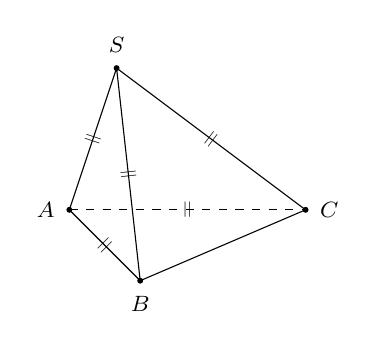
\begin{tikzpicture}[scale=0.6, font=\footnotesize,>=stealth]
			\path
			(0,0) coordinate (A)
			(5,0) coordinate (C)
			(1.5,-1.5) coordinate (B)
			(1,3) coordinate (S)
			;
			\draw (S)--(A)node[midway,sloped,scale=0.7]{$||$}--(B)node[midway,sloped,scale=0.7]{$||$}--(C)--(S)node[midway,sloped,scale=0.7]{$||$} (S)--(B)node[midway,sloped,scale=0.7]{$||$};
			\draw[dashed](A)--(C)node[midway,sloped,scale=0.7]{$||$};
			\foreach \x/\g in {A/180,S/90,C/0,B/-90}\draw[fill=black] (\x) circle (.05) +(\g:.5)node{\footnotesize$\x$};
	\end{tikzpicture}}
	\loigiai{
		\immini{Ta có
			\begin{align*}	
				\cos \left(\vec{S C}, \vec{A B}\right) &\ =\dfrac{\vec{S C} \cdot \vec{A B}}{\left|\vec{S C}\right| \cdot\left|\vec{A B}\right|}=\dfrac{\left(\vec{S A}+\vec{A C}\right) \cdot \vec{A B}}{a^2} \\
				&\ =\dfrac{\vec{S A} \cdot \vec{A B}+\vec{A C} \cdot \vec{A B}}{a^2}.
			\end{align*}
			Từ giả thiết suy ra $S A B$ là tam giác đều và $A B C$ là tam giác vuông cân tại $A$. Từ đó ta tính được
			$\vec{S A} \cdot \vec{A B}=a\cdot a \cdot \cos 120^{\circ}=-\dfrac{a^2}{2}$ và $\vec{A C} \cdot \vec{A B}=0$.\\
			Suy ra $\cos \left(\vec{S C}, \vec{A B}\right)=-\dfrac{1}{2}$.\\
			Vậy $\cos \left(\vec{S C}, \vec{A B}\right)=120^{\circ}$.
		}{
			\begin{tikzpicture}[scale=0.7, font=\footnotesize,>=stealth]
				\path
				(0,0) coordinate (A)
				(5,0) coordinate (C)
				(1.5,-1.5) coordinate (B)
				(1,3) coordinate (S)
				;
				\draw (S)--(A)node[midway,sloped,scale=0.7]{$||$}--(B)node[midway,sloped,scale=0.7]{$||$}--(C)--(S)node[midway,sloped,scale=0.7]{$||$} (S)--(B)node[midway,sloped,scale=0.7]{$||$};
				\draw[dashed](A)--(C)node[midway,sloped,scale=0.7]{$||$};
				\foreach \x/\g in {A/180,S/90,C/0,B/-90}\draw[fill=black] (\x) circle (.05) +(\g:.5)node{\footnotesize$\x$};
				\draw pic[draw,angle radius=0.3cm]{right angle=B--S--C};
		\end{tikzpicture}}
	}
\end{ex} \cham{7}

\begin{ex}
	\immini[thm]{Cho tứ diện $OABC$ có các cạnh $OA$, $OB$, $OC$ đôi một vuông góc và $OA=OB=OC=1$. Gọi $M$ là trung điểm của cạnh $AB$. Tính góc giữa hai vectơ $\vec{OM}$ và $\vec{AC}$.
		\haicot
		{$90^\circ$}
		{\True $120^\circ$}
		{$60^\circ$}
		{$30^\circ$}}{
		\begin{tikzpicture}[scale=0.4, font=\footnotesize, line join=round, line cap=round]
			\foreach \x\y\t in {0/0/O,3/-3.6/A,7/2/B,0.3/5/C} \coordinate (\t) at (\x,\y);
			\draw (O)--(C)--(B)--(A)--(O);
			\coordinate (M) at ($(A)!1/2!(B)$);
			\draw[-stealth,thick] (A)--(C);
			\draw[-stealth,dashed,thick] (O)--(M);
			\draw[dashed] (O)--(B);
			\foreach \t/\g in {A/-90,B/0,C/90,O/180,M/0} \draw (\t) node[shift={(\g:10pt)}]{$\t$};
	\end{tikzpicture}}
	\loigiai{
		\immini{Đặt $\vec{OA}=\vec{a}$, $\vec{OB}=\vec{b}$, $\vec{OC}=\vec{c}$. \\
			Khi đó, $\left| \vec{a} \right| = \left| \vec{b} \right| = \left| \vec{c} \right| = 1$ và $\vec{a} \cdot \vec{b} = \vec{a} \cdot \vec{c} = \vec{b} \cdot \vec{c} = 0$.\\
			Ta có $\cos \left(\vec{OM},\vec{AC} \right) = \dfrac{\vec{OM} \cdot \vec{AC}}{\left| \vec{OM} \right| \cdot \left| \vec{AC} \right|}$.\\
			Mặt khác do $\vec{OM} = \dfrac{1}{2} \left(\vec{OA}+\vec{OB} \right) = \dfrac{1}{2} \left(\vec{a}+\vec{b} \right)$\\
			và $\vec{AC} = \vec{OC} - \vec{OA} = \vec{c} - \vec{a}$\\
			nên $\begin{aligned}[t]
				\vec{OM} \cdot \vec{AC} &=\dfrac{1}{2} \left(\vec{a}+\vec{b} \right) \cdot \left(\vec{c}-\vec{a} \right) \\
				&=\dfrac{1}{2} \left(\vec{a} \cdot \vec{c}-\vec{a}^2+ \vec{b} \cdot \vec{c} - \vec{b} \cdot \vec{a} \right) = -\dfrac{1}{2}. \\
			\end{aligned}$
		}
		{\begin{tikzpicture}[scale=0.45, font=\footnotesize, line join=round, line cap=round]
				\foreach \x\y\t in {0/0/O,3/-3.6/A,7/2/B,0.3/5/C} \coordinate (\t) at (\x,\y);
				\draw (O)--(C)--(B)--(A)--(O);
				\coordinate (M) at ($(A)!1/2!(B)$);
				\draw[-stealth,red,very thick] (A)--(C);
				\draw[-stealth,dashed,red,very thick] (O)--(M);
				\draw[dashed] (O)--(B);
				\foreach \t/\g in {A/-90,B/0,C/90,O/180,M/0} \draw (\t) node[shift={(\g:10pt)}]{$\t$};
		\end{tikzpicture}}
		Ta lại có $\left| \vec{OM} \right| = OM =\dfrac{\sqrt{2}}{2}$, $\left| \vec{AC} \right| = AC = \sqrt{2}$. \\
		Do đó $\cos \left(\vec{OM},\vec{AC} \right) = \dfrac{\vec{OM} \cdot \vec{AC}}{\left| \vec{OM} \right| \cdot \left| \vec{AC} \right|} = \dfrac{\dfrac{-1}{2}}{\dfrac{\sqrt{2}}{2} \cdot \sqrt{2}} = \dfrac{-1}{2}$. \\
		Vậy $\left( \vec{OM}, \vec{AC}\right) = 120^\circ$.
	}
\end{ex} \cham{7}

\begin{ex}%[2H2V1-4]%[Dự án đề kiểm tra Toán khối 12 GHKI NH24-25- Đợt 3 - Nhật Thiện]%[Trường THPT LÝ THƯỜNG KIỆT - HCM]
	\immini[thm]{Có ba lực cùng tác động vào một vật. Hai trong ba lực này hợp với nhau một góc $110^\circ$ và có độ lớn lần lượt là $30$ N, $25$ N. Lực thứ ba vuông góc với mặt phẳng tạo bởi hai lực đã cho và có độ lớn là $10$ N. Tính độ lớn hợp lực của ba lực đã cho. (Kết quả làm tròn đến hàng phần mười)
	\haicot
	{$30,6$ N}
	{\True $33,3$ N}
	{$32,7$ N}
	{$35,2$ N}
}{
\begin{tikzpicture}[scale=1, font=\footnotesize, line join=round, line cap=round, >=stealth]
	\path 
	(0,0) coordinate (O)
	+(-2,-1) coordinate (B)
	+(4,0) coordinate (A)
	+(0,3) coordinate (C)
	($(A)+(B)-(O)$) coordinate (D)
	($(C)+(D)-(O)$) coordinate (E)
	;
	\draw[->] (O)--node[midway,above right]{$\vec{F}_1$}(A);
	\draw[->] (O)--node[midway,above]{$\vec{F}_2$}(B);
	\draw[->] (O)--node[midway,left]{$\vec{F}_3$}(C);
	\draw[->] (O)--(D);
	\draw[->] (O)--(E);
	\draw[dashed] (A)--(D)--(B) (D)--(E)--(C);
	\foreach \p/\r in {A/90,B/-120,O/150,D/-90,E/60,C/90}
	\fill (\p) circle (1pt) node[shift={(\r:3mm)}]{$\p$};
\end{tikzpicture}}
	\loigiai{
		\immini{Gọi $\vec{F}_1$, $\vec{F}_2$, $\vec{F}_3$ lần lượt là ba lực tác động vào vật như hình vẽ.\\
			Ta có $\vec{F}_1=\vec{OA}$, $\vec{F}_2=\vec{OB}$, $\vec{F}_3=\vec{OC}$.\\
			Và $OA=30$, $OB=25$, $OC=10$.\\
			Dựng hình bình hành $OADB$, khi đó $\vec{OA}+\vec{OB}=\vec{OD}$.\\
			Suy ra $$OD^2=OA^2+OB^2+2\cdot OA\cdot OB\cdot \cos \left(\vec{OA},\vec{OB}\right).$$
			Dựng hình bình hành $ODEC$, khi đó hợp lực của ba lực đã cho là 
			$$F=\vec{F}_1+\vec{F}_2+\vec{F}_3=\vec{OA}+\vec{OB}+\vec{OC}=\vec{OE}.$$
			Do $OE\perp (OADB)$ nên }
		{
			\begin{tikzpicture}[scale=1, font=\footnotesize, line join=round, line cap=round, >=stealth]
				\path 
				(0,0) coordinate (O)
				+(-2,-1) coordinate (B)
				+(4,0) coordinate (A)
				+(0,3) coordinate (C)
				($(A)+(B)-(O)$) coordinate (D)
				($(C)+(D)-(O)$) coordinate (E)
				;
				\draw[->] (O)--node[midway,above right]{$\vec{F}_1$}(A);
				\draw[->] (O)--node[midway,above]{$\vec{F}_2$}(B);
				\draw[->] (O)--node[midway,left]{$\vec{F}_3$}(C);
				\draw[->] (O)--(D);
				\draw[->] (O)--(E);
				\draw[dashed] (A)--(D)--(B) (D)--(E)--(C);
				\foreach \p/\r in {A/90,B/-120,O/120,D/-90,E/60,C/90}
				\fill (\p) circle (1pt) node[shift={(\r:3mm)}]{$\p$};
			\end{tikzpicture}
		}
		\noindent $OE=\sqrt{OC^2+OD^2}=\sqrt{OC^2+OA^2+OB^2+2\cdot OA\cdot OB\cdot \cos \left(\vec{OA},\vec{OB}\right)}\approx 33{,}3.$
	}
\end{ex}
\cham{9}
\Closesolutionfile{ans}

\ind{PHẦN II.} \inden{Câu trắc nghiệm đúng sai. Trong mỗi ý a), b), c), d) ở mỗi câu, học sinh chọn đúng hoặc sai.}\\
\Opensolutionfile{ans}[ans/2H2-B1-d2-2]
\begin{ex}%[2H2H1-3]
	Trong không gian, cho hai véc-tơ $\vec{a}$ và $\vec{b}$ cùng có độ dài bằng $1$. Biết rằng góc giữa hai véc-tơ đó là $45^{\circ}$.
	\choiceTF
	{\True $\vec{a}\cdot \vec{b}=\dfrac{\sqrt{2}}{2}$}
	{\True $\left( \vec{a}+3 \vec{b}\right) \cdot\left( \vec{a}-2 \vec{b}\right)=-5+\dfrac{\sqrt{2}}{2}$}
	{$\left| \vec{a}+ \vec{b}\right|=2+\sqrt{2} $}
	{$\left| \vec{a}-\sqrt{2}\vec{b}\right|=0$}
	\loigiai{
		\begin{enumerate}[a)]
			\item $\vec{a}\cdot \vec{b}=\left| \vec{a}\right|\cdot \left| \vec{b}\right|\cos \left(\vec{a},\vec{b} \right)=\dfrac{\sqrt{2}}{2}$.
			\item $\left( \vec{a}+3 \vec{b}\right) \cdot\left( \vec{a}-2 \vec{b}\right)=\left| \vec{a}\right|^2+\cdot\vec{a}\cdot \vec{b}-6\left| \vec{b}\right|^2 =1+\cdot\dfrac{\sqrt{2}}{2}-6=-5+\dfrac{\sqrt{2}}{2} $.
			\item $\left( \vec{a}+ \vec{b}\right)^2= \vec{a}^2+2\vec{a}\cdot \vec{b}+\vec{b}^2=1+2\cdot\dfrac{\sqrt{2}}{2}+1=2+\sqrt{2}$. Suy ra $\left| \vec{a}+ \vec{b}\right|=\sqrt{2+\sqrt{2}}$.
			\item $\left( \vec{a}-\sqrt{2} \vec{b}\right)^2= \vec{a}^2+2\sqrt{2}\vec{a}\cdot \vec{b}+2\vec{b}^2=1+2\sqrt{2}\cdot\dfrac{\sqrt{2}}{2}+2=2$. Suy ra $\left| \vec{a}- \sqrt{2}\vec{b}\right|=\sqrt{2}$.
		\end{enumerate}
	}
\end{ex} \cham{14}

\begin{ex}%[2H2H1-3]%[Dự án đề kiểm tra môn Toán khối 12 GHKI NH24-25 - Đợt 3 - Thành Đức Trung]%[THPT Tam Phú - TP Hồ Chí Minh]
	\immini
	{
		Cho hình chóp $S.ABCD$ có đáy là hình vuông cạnh $2a$. Biết $SA=2a$ và $SA$ vuông góc với mặt phẳng $(ABCD)$. $M$ là trung điểm $SB$.
		\choiceTF
		{Tích vô hướng của hai véc-tơ $\overrightarrow{SD}$ và $\overrightarrow{CD}$ là $-1$}
		{\True Độ dài của véc-tơ $\overrightarrow{AM}$ là $a\sqrt{2}$}
		{Góc giữa hai véc-tơ $\overrightarrow{AC}$ và $\overrightarrow{CD}$ bằng $45^\circ$}
		{\True Tích vô hướng của hai véc-tơ $\overrightarrow{SC}$ và $\overrightarrow{AB}$ là $4a^2$}
	}
	{
		\begin{tikzpicture}[scale=1, font=\footnotesize, line join=round, line cap=round, >=stealth]
			\path
			(0,0)coordinate(A)
			(-1.5,-1.5)coordinate(B)
			(4,0)coordinate(D)
			(0,2.5)coordinate(S)
			($(B)+(D)-(A)$)coordinate(C)
			;
			\draw(S)--(B) (S)--(C) (S)--(D) (C)--(D) (B)--(C);
			\draw[dashed](A)--(B) (A)--(D) (S)--(A);
			\foreach \p/\q in {S/90, A/-180, B/-90, C/-90, D/0} \fill[black] (\p) circle (1pt) ($(\p)+(\q:2.5mm)$) node{$\p$};
		\end{tikzpicture}
	}
	\loigiai
	{
		\begin{center}
			\begin{tikzpicture}[scale=1, font=\footnotesize, line join=round, line cap=round, >=stealth]
				\path
				(0,0)coordinate(A)
				(-1.5,-1.5)coordinate(B)
				(4,0)coordinate(D)
				(0,3.5)coordinate(S)
				($(B)+(D)-(A)$)coordinate(C)
				($(S)!0.5!(B)$)coordinate(M)
				;
				\draw(S)--(B) (S)--(C) (S)--(D) (C)--(D) (B)--(C);
				\draw[dashed](A)--(B) (A)--(D) (A)--(C) (S)--(A)--(M);
				\foreach \p/\q in {S/90, A/-180, B/-90, C/-90,M/180, D/0} \fill[black] (\p) circle (1pt) ($(\p)+(\q:2.5mm)$) node{$\p$};
			\end{tikzpicture}
		\end{center}
		\begin{itemchoice}
			\itemch Sai vì ta có $\heva{ & CD\perp AD\subset (SAD) \\ & CD\perp SA\subset (SAD)} \Rightarrow CD\perp SD \subset (SAD)$.\\
			Suy ra tích vô hướng của hai véc-tơ $\overrightarrow{SD}$ và $\overrightarrow{CD}$ là $0$.
			\itemch Xét tam giác $SAB$ vuông tại $A$. \\
			Suy ra $AM=\dfrac{1}{2}SB=\dfrac{1}{2}\sqrt{SA^2+AB^2}=\dfrac{1}{2}\sqrt{(2a)^2+(2a)^2}=a\sqrt{2}$.\\
			Vậy độ dài véc-tơ $\overrightarrow{AM}=a\sqrt{2}$.
			\itemch Ta có $\left(\overrightarrow{AC},\overrightarrow{CD}\right)=180^\circ -\left(\overrightarrow{CA},\overrightarrow{CD}\right)=180^\circ -\widehat{ACD}=180^\circ-45^\circ=135^\circ$
			\itemch Ta có $\overrightarrow{SC}\cdot \overrightarrow{AB}=\left(\overrightarrow{AC}-\overrightarrow{AS}\right)\cdot \overrightarrow{AB}=\overrightarrow{AC}\cdot \overrightarrow{AB}-\overrightarrow{AS}\cdot \overrightarrow{AB}=AC\cdot AB\cdot \cos \widehat{BAC}-0$\\
			Suy ra $\overrightarrow{SC}\cdot \overrightarrow{AB}=\sqrt{(2a)^2+(2a)^2}\cdot 2a \cdot \cos 45^\circ=4a^2$.
		\end{itemchoice}
	}
\end{ex}
\cham{12}
\begin{ex}%[2H2H1-3]%[2-TN-DS-TLN-THPT-NguyenThaiBinh-GHKI-NH23-24]%[Hector Tran]
	\immini{Cho hình lập phương $ABCD.A'B'C'D'$ có cạnh bằng $a$. Xét tính đúng sai của các mệnh đề sau.
	\choiceTF
	{\True Gọi $M$ là trung điểm của $BC$. Độ dài véctơ $\overrightarrow {A'M}$ bằng $\dfrac{3a}{2}$}
	{\True $\overrightarrow {AC'}=\overrightarrow {AB}+\overrightarrow {AD}+\overrightarrow {AA'}$}
	{$\overrightarrow {A'B}=\overrightarrow {AB}+\overrightarrow {AA'}$}
	{Góc giữa véctơ $\overrightarrow {BA'}$ và véctơ $\overrightarrow {A'C'}$ bằng $60^\circ$}
}{
\begin{tikzpicture}[scale=1, line join=round, line cap=round]
	\tkzDefPoints{0/0/A,-1.3/-1.1/B,2/-1.1/C}
	\coordinate (D) at ($(A)+(C)-(B)$);
	\coordinate (A') at ($(A)+(0,2.5)$);
	\tkzDefPointsBy[translation=from A to A'](B,C,D){B'}{C'}{D'}
	\tkzDrawPolygon(A',B',B,C,D,D')
	\tkzDrawSegments(B',C' C',D' C,C')
	\tkzDrawSegments[dashed](A,B A,D A,A')
	\tkzDrawPoints[fill=black,size=4](A,B,D,C,A',B',C',D')
	\tkzLabelPoints[above](A',D')
	\tkzLabelPoints[below](A,B,C)
	\tkzLabelPoints[left](B')
	\tkzLabelPoints[right](C',D)
\end{tikzpicture}}
	\loigiai{
		\begin{center}
			\begin{tikzpicture}[scale=0.6, font=\footnotesize,line join=round, line cap=round, >=stealth]
				\path 
				(0,0) coordinate (A)
				++(-120:3) coordinate (D)
				++(0:5) coordinate (C)
				($(A)+(C)-(D)$) coordinate (B)
				($(A)!1/2!(C)$) coordinate (O)
				($(B)!1/2!(C)$) coordinate (M)
				;
				\foreach \i in {A,B,C,D}{
					\coordinate (\i') at ($(\i)+(0,4)$);
				}
				\draw (A')--(B')--(C')--(D')--cycle;
				\draw (B)--(B') (C)--(C') (D)--(D')  (B)--(C)--(D) (A')--(C');
				\draw[dashed,thin](B)--(A)--(A')--(M) (C)--(A)--(D) (A)--(M) (A')--(B) (A)--(C');
				\pic[draw,angle eccentricity=1.8,angle radius=2mm]{right angle=M--A--A'};
				\foreach \i/\g in {A'/90,B'/90,C'/90,D'/90,A/-90,B/-90,C/-90,D/-90,M/-90}
				\fill[black] (\i) circle(1pt)+(\g:5mm)node[scale=1]{$\i$};
			\end{tikzpicture}
		\end{center}
		\begin{itemchoice}
			\itemch \textbf{Đúng}. Ta có $\big|\overrightarrow {A'M}\big|=\sqrt{AA'^2+AM^2}=\sqrt{a^2+a^2+\dfrac{a^2}{4}}=\dfrac{3a}{2}$.
			\itemch \textbf{Đúng}. Theo quy tắc hình hộp ta có $\overrightarrow {AC'}=\overrightarrow {AB}+\overrightarrow {AD}+\overrightarrow {AA'}$.
			\itemch \textbf{Sai}. Ta có $\overrightarrow {AB}+\overrightarrow {AA'}=\overrightarrow {AB'}\ne \overrightarrow {A'B}$.
			\itemch \textbf{Sai}. $\left(\overrightarrow {BA'},\overrightarrow {A'C'}\right)=180^\circ-\widehat {BA'C'}=120^\circ$ ($\triangle A'BC'$ có ba cạnh $A'B=BC'=A'C=a\sqrt{2}$ là tam giác đều).
		\end{itemchoice}
	}
\end{ex}
\cham{10}

\begin{ex}
	\immini{Cho tứ diện đều ${SBCD}$ có cạnh bằng ${5 a}$. Gọi ${E}$ là trung điểm của cạnh ${BC}$. Gọi ${H}$ là trọng tâm tam giác ${BCD}$. Xét tính đúng-sai của các khẳng định sau.
	\choiceTF
	{ $(\overrightarrow{HB},\overrightarrow{CH}) = 120^\circ$ }
	{ \True $\overrightarrow{SB}.\overrightarrow{CD}=0$ }
	{ \True $\overrightarrow{SB}+\overrightarrow{CD}+\overrightarrow{BC}+\overrightarrow{DS}=\overrightarrow{0}$ }
	{ \True $\overrightarrow{SB}.\overrightarrow{CS}=- \dfrac{25 a^{2}}{2}$ }
}{
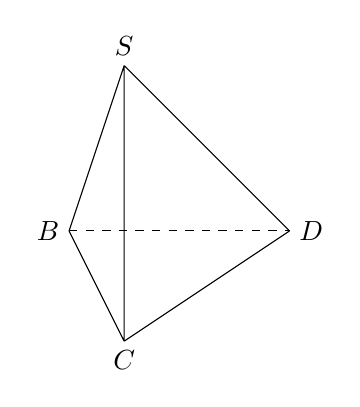
\begin{tikzpicture}[scale=0.7]
	\coordinate (B) at (0,0)   node at (B) [left] {$B$};
	\coordinate (C) at (1,-2) node at (C) [below] {$C$};
	\coordinate (D) at (4,0)   node at (D) [right] {$D$};
	\coordinate (S) at (1,3)   node at (S) [above] {$S$};
	\draw [dashed] (B)--(D) ; 
	\draw (B)--(C) (C)--(D) (S)--(B) (S)--(C) (S)--(D);
\end{tikzpicture}}
	\loigiai{ 
		
		
		a) Khẳng định đã cho là khẳng định sai.
		
		$(\overrightarrow{HB},\overrightarrow{CH})=180^\circ-(\overrightarrow{HB},\overrightarrow{HC})=180^\circ - 120^\circ=60^\circ$
		
		b) Khẳng định đã cho là khẳng định đúng.
		
		Gọi ${N}$ là trung điểm của ${CD}$.
		
		$CD\bot BN, CD\bot SN \Rightarrow  CD\bot (SBN) \Rightarrow CD\bot SB$.
		
		Vậy $\overrightarrow{SB}.\overrightarrow{CD}=0$.
		
		c) Khẳng định đã cho là khẳng định đúng.
		
		$\overrightarrow{SB}+\overrightarrow{CD}+\overrightarrow{BC}+\overrightarrow{DS}=\overrightarrow{SB}+\overrightarrow{BC}+\overrightarrow{CD}+\overrightarrow{DS}=\overrightarrow{SS}=\overrightarrow{0}$.
		
		d) Khẳng định đã cho là khẳng định đúng.
		
		$\overrightarrow{SB}.\overrightarrow{CS}=SB.CS.\cos(\overrightarrow{SB}, \overrightarrow{CS})$$=5 a.5 a.- \frac{1}{2}=- \frac{25 a^{2}}{2}$.
		
		
}\end{ex}

\cham{10}
\begin{ex}
	\immini{
		Một chất điểm ở vị trí đỉnh $A$ của hình lập phương $ABCD.A'B'C'D'$. Chất điểm chịu tác động bởi ba lực $\vec{a}$, $\vec{b}$, $\vec{c}$ lần lượt cùng hướng với $\vec{AD}$, $\vec{AB}$ và $\vec{AC'}$ như hình vẽ. Độ lớn của các lực $\vec{a}$, $\vec{b}$ và $\vec{c}$ tương ứng là $10$ N, $10$ N và $20$ N. 
		\choiceTF
		{$\vec{a}+\vec{b}=\vec{c}$}
		{$\big|\vec{a}+\vec{b}\big|=20$ (N)}
		{\True $\big|\vec{a}+\vec{c}\big|=\big|\vec{b}+\vec{c}\big|$}
		{\True $\big|\vec{a}+\vec{b}+\vec{c}\big|=32{,}59$ (N) (\textit{làm tròn kết quả đến hàng phần mười})}
	}{\hspace{0.5cm}
		\begin{tikzpicture}[line join=round, line cap = round, >=stealth, scale=0.65,font=\footnotesize]
			\path 
			(0,0) coordinate (A') 
			(-1.5,-1.5) coordinate (D') 
			(2,-1.5) coordinate (C') 
			(3.5,0) coordinate (B') 
			(0,3.5) coordinate (A) 
			($(A)+(B')-(A')$) coordinate (B) 
			($(A)+(C')-(A')$) coordinate (C)
			($(A)+(D')-(A')$) coordinate (D)
			($(A)!1/2!(D)$) coordinate (M)
			($(A)!1/2!(B)$) coordinate (N)
			($(A)!1/2!(C')$) coordinate (P)
			; 
			\draw[->,thick](A)--node [left]{$\vec{a}$}(M);
			\draw[->,thick](A)--node [above]{$\vec{b}$}(N);
			\draw[->,thick](A)--node[right]{$\vec{c}$}(P);
			\draw[dashed] (D')--(A')--(B') (A')--(A)--(C'); 
			\draw (D)--(C)--(B)--(A)--(D)--(D')--(C')--(C) (C')--(B')--(B); 
			\draw pic[draw,angle eccentricity=1.2,angle radius=0.25cm]{right angle= D--A--B};
			\foreach \x/\g in {A/90,B/80,C/-40,D/110,A'/160,B'/-65,C'/-90,D'/-100} \fill[black](\x) circle (1pt) ($(\x)+(\g:3mm)$)node{$\x$}; 
		\end{tikzpicture} 
	}
	\loigiai{
		Từ giả thiết, ta có $\vec{a} \perp \vec{b};\cos\left(\vec{a},\vec{c}\right)= \cos \widehat{DAC'}= \dfrac{1}{\sqrt3}; \cos \left(\vec{b},\vec{c}\right)= \cos \widehat{BAC'}= \dfrac{1}{\sqrt3}$.\\
		\begin{enumerate}[a)]
			\item Giả sử $\vec{a}+\vec{b}=\vec{d}$. Theo quy tắc hình bình hành thì $\vec{d}$ cùng hướng với $\vec{AC}$. Suy ra $\vec{a}+\vec{b}\ne \vec{c}$
			\item  $\big|\vec{a}+\vec{b}\big|=10\sqrt{2}$ (đường chéo hình vuông cạnh bằng 10).
			\item  Ta có
			\begin{itemize}
				\item [$\bullet$] $\big(\vec{a}+\vec{c}\big)^2=|\vec{a}|^2+2\vec{a} \cdot \vec{c}+|\vec{c}|^2=10^2+2.10.20.\dfrac{1}{\sqrt{3}}+20^2=500+\dfrac{400\sqrt{3}}{3}$.\\
				Suy ra $\big|\vec{a}+\vec{c}\big|=\sqrt{500+\dfrac{400\sqrt{3}}{3}}$.
				\item [$\bullet$] $\big(\vec{b}+\vec{c}\big)^2=|\vec{b}|^2+2\vec{b} \cdot \vec{c}+|\vec{c}|^2=10^2+2.10.20.\dfrac{1}{\sqrt{3}}+20^2=500+\dfrac{400\sqrt{3}}{3}$.\\
				Suy ra $\big|\vec{b}+\vec{c}\big|=\sqrt{500+\dfrac{400\sqrt{3}}{3}}$.
			\end{itemize}
			Vậy $\big|\vec{a}+\vec{c}\big|=\big|\vec{b}+\vec{c}\big|$.
			\item Giả sử lực tổng hợp là $\vec{m}$, tức là $\vec{m}=\vec{a}+\vec{b}+\vec{c}$.\\
			Do đó
			\allowdisplaybreaks 
			\begin{eqnarray*}
				\vec{m}=\vec{a}+\vec{b}+\vec{c} &\Leftrightarrow& \left|\vec{m}\right|^2= \left(\vec{a}+\vec{b}+\vec{c}\right)^2\\
				&\Leftrightarrow& \left|\vec{m}\right|^2= \vec{a}^2+\vec{b}^2+\vec{c}^2+2\vec{a}\cdot\vec{b}+2\vec{b}\cdot\vec{c}+2\vec{c}\cdot\vec{a}\\
				&\Leftrightarrow& \left|\vec{m}\right|^2= 10^2+10^2+20^2+0+2\cdot 10\cdot 20 \cdot \dfrac{1}{\sqrt3} +2\cdot 10\cdot 20 \cdot \dfrac{1}{\sqrt3}\\
				&\Leftrightarrow& \left|\vec{m}\right|^2= 10^2+10^2+20^2+0+2\cdot 10\cdot 20 \cdot \dfrac{1}{\sqrt3} +2\cdot 10\cdot 20 \cdot \dfrac{1}{\sqrt3}\\
				&\Leftrightarrow& \left|\vec{m}\right| \approx 32{,}59.
			\end{eqnarray*}
			Vậy cường độ hợp lực của $\vec{a}$, $\vec{b}$ và $\vec{c}$ là $\approx 32{,}59$ (N).
		\end{enumerate}
		
	}
\end{ex} \cham{12}



\Closesolutionfile{ans}
